\documentclass{article}

\usepackage{amsmath}
\usepackage{upgreek}
\usepackage{dsfont}
\usepackage{mdframed}
%margin package
\usepackage[margin=1in,includefoot]{geometry}
%graphics packages
\usepackage{graphicx}
\usepackage{float}
%pseudocode packages
\usepackage{amsmath}
\usepackage{algorithm}
\usepackage[noend]{algpseudocode}
\usepackage{listings}

\begin{document}

\begin{enumerate}
%%%%%%%%%%%%%%%%%%%%%%%%%%%%%%%%%%%%%%%%%%%%%%%%%%%%%%%%%%%%%%%%%%%%%%%%%%%%%%%%%%%%%%%%
%% GRID GENERATION
%%%%%%%%%%%%%%%%%%%%%%%%%%%%%%%%%%%%%%%%%%%%%%%%%%%%%%%%%%%%%%%%%%%%%%%%%%%%%%%%%%%%%%%%

\item GRID GENERATION

En esta sección explicaremos el problema al cu\'al analizaremos para el precondicionamiento, el cu\'al
es el de la generaci\'on de mallas.

\begin{itemize}

%%%%%%%%%%%%%%%%%%%%%%%%%%%%%%%%%%%%%%%%%%%%%%%%%%%%%%%%%%%%%%%%%%%%%%%%%%%%%%%%%%%%%%%%%%%%%%%%%%%%%%%%%%%%%%%%%%%%%%

\item[a)] \textbf{ ¿ Qu\'e es la generaci\'on de mallas ? }
\\
%% Breve explicación de en que consiste grid generation y para que se usa %%%%%%%%%%%%%%%%

Lorem ipsum dolor sit amet, consectetur adipiscing elit, sed do eiusmod tempor incididunt ut labore et dolore magna aliqua. Ut enim ad minim veniam, quis nostrud exercitation ullamco laboris nisi ut aliquip ex ea commodo consequat. Duis aute irure dolor in reprehenderit in voluptate velit esse cillum dolore eu fugiat nulla pariatur. Excepteur sint occaecat cupidatat non proident, sunt in culpa qui officia deserunt mollit anim id est laborum.
\\
%%%%%%%%%%%%%%%%%%%%%%%%%%%%%%%%%%%%%%%%%%%%%%%%%%%%%%%%%%%%%%%%%%%%%%%%%%%%%%%%%%%%%%%%%%

%% Ejemplos -> imágenes sobre generación estructurada y no estructurada, y una breve explicación de ambas

Lorem ipsum dolor sit amet, consectetur adipiscing elit, sed do eiusmod tempor incididunt ut labore et dolore magna aliqua. Ut enim ad minim veniam, quis nostrud exercitation ullamco laboris nisi ut aliquip ex ea commodo consequat. Duis aute irure dolor in reprehenderit in voluptate velit esse cillum dolore eu fugiat nulla pariatur. Excepteur sint occaecat cupidatat non proident, sunt in culpa qui officia deserunt mollit anim id est laborum.
\\
%%%%%%%%%%%%%%%%%%%%%%%%%%%%%%%%%%%%%

%% Mencionar sobre nuestro caso, el estructurado 

Lorem ipsum dolor sit amet, consectetur adipiscing elit, sed do eiusmod tempor incididunt ut labore et dolore magna aliqua. Ut enim ad minim veniam, quis nostrud exercitation ullamco laboris nisi ut aliquip ex ea commodo consequat. Duis aute irure dolor in reprehenderit in voluptate velit esse cillum dolore eu fugiat nulla pariatur. Excepteur sint occaecat cupidatat non proident, sunt in culpa qui officia deserunt mollit anim id est laborum.
\\
%%%%%%%%%%%%%%%%%%%%%%%%%%%%%%%%%%%%%%%%%%%%%%%%%

%% Structured grid generation methods
\item[b)] \textbf{ M\'etodos para generaci\'on de mallas estructuradas }
\\
%% Breve intro a métodos algebráicos y basados en PDEs %%%%%%%%%%%%%%

Lorem ipsum dolor sit amet, consectetur adipiscing elit, sed do eiusmod tempor incididunt ut labore et dolore magna aliqua. Ut enim ad minim veniam, quis nostrud exercitation ullamco laboris nisi ut aliquip ex ea commodo consequat. Duis aute irure dolor in reprehenderit in voluptate velit esse cillum dolore eu fugiat nulla pariatur. Excepteur sint occaecat cupidatat non proident, sunt in culpa qui officia deserunt mollit anim id est laborum.
\\


	\begin{itemize}
		%% Tal vez también se pueda mencionar los de mapeo simple, los que haces cambio de variable y ya
		% \item M\'etodos de mapeo

		%% Métodos algebraicos de interpolación %%%%%%%%%%%%%%%%%%%%%%%%
		\item M\'etodos algebraicos basados en interpolaci\'on
		\\
		Lorem ipsum dolor sit amet, consectetur adipiscing elit, sed do eiusmod tempor incididunt ut labore et dolore magna aliqua. Ut enim ad minim veniam, quis nostrud exercitation ullamco laboris nisi ut aliquip ex ea commodo consequat. Duis aute irure dolor in reprehenderit in voluptate velit esse cillum dolore eu fugiat nulla pariatur. Excepteur sint occaecat cupidatat non proident, sunt in culpa qui officia deserunt mollit anim id est laborum.	
		\\
		%%%%%%%%%%%%%%%%%%%%%%%%%%%%%%%%%%%%%%%%%%%%%%%%%%%%%%%%%%%%%%%%

		%% Métodos basados en PDEs %%%%%%%%%%%%%%%%%%%%%%%%%%%%%%%%%%%%%
		%% Mencionar tal vez el hiperbólico, pero hacer énfasis en el
		%% elíptico, y mencionar que es el que usamos en nuestro caso
		\item M\'etodos basados en PDEs
		\\
		Lorem ipsum dolor sit amet, consectetur adipiscing elit, sed do eiusmod tempor incididunt ut labore et dolore magna aliqua. Ut enim ad minim veniam, quis nostrud exercitation ullamco laboris nisi ut aliquip ex ea commodo consequat. Duis aute irure dolor in reprehenderit in voluptate velit esse cillum dolore eu fugiat nulla pariatur. Excepteur sint occaecat cupidatat non proident, sunt in culpa qui officia deserunt mollit anim id est laborum.	
		%%%%%%%%%%%%%%%%%%%%%%%%%%%%%%%%%%%%%%%%%%%%%%%%%%%%%%%%%%%%%%%%

	\end{itemize}


%%%%%%%%%%%%%%%%%%%%%%%%%%%%%%%%%%%%%%%%%%%%%%%%%%%%%%%%%%%%%%%%%%%%

%% Our implementation %%%%%%%%%%%%%%%%%%%%%%%%%%%%%%%%%%%%%%%%%%%%%%
\item[c)] \textbf{ Sobre los m\'etodos usados }
\\
	En nuestra implementaci\'on decidimos seguir el procedimiento propuesto en varios libros y papers. Seguimos el 
	siguiente procedimiento: 

	\begin{itemize}
		\item[*] \textbf{ Uso de un generador algebraico }
		\\
		Usamos un generador basado en la Interpolaci\'on Transfinita. La malla generada se usar\'a como condici\'on 
		inicial para nuestro generador basado en PDEs.
		%%%%
		\item[*] \textbf{ Discretizaci\'on de las ecuaciones del generador el\'iptico }
		\\
		El generador basado en PDEs usado es el El\'iptico, cuyas ecuaciones son discretizadas y formadas en un 
		m\'etodo iterativo para calcular un grid por medio de la Iteraci\'on de Picard.
		%%%%
		\item[*] \textbf{ Refinamiento de la malla }
		\\ En este \'ultimo paso usamos el generador El\'iptico discretizado para as\'i poder refinar la malla
		inicial generada por el generador algebraico.
	\end{itemize}

	Acontinuaci\'on pasamos a describir los m\'etodos usados.

	\begin{itemize}

		\item[a)] \textbf{ M\'etodo algebraico de interpolaci\'on transfinita }
		\\
		En nuestra implementaci\'on usamos el generador algebraico basado en Interpolaci\'on Transfinita. Este puede ser formulado como sigue :
		%
		\begin{gather*}
			x( \xi, \eta ) = ( 1 - \xi ) x_{l} + \xi x_{r} + ( 1 - \eta ) x_{b} + \eta x_{t} - \hdots \\
							 ( 1 - \eta ) ( 1 - \xi ) x_{b}(0) - ( 1 - \xi ) \eta x_{t}(0) - \hdots \\
							 ( 1 - \eta ) \xi x_{b}(1) - \eta \xi x_{t}(1)
			\\
			y( \xi, \eta ) = ( 1 - \xi ) y_{l} + \xi y_{r} + ( 1 - \eta ) y_{b} + \eta y_{t} - \hdots \\
							 ( 1 - \eta ) ( 1 - \xi ) y_{b}(0) - ( 1 - \xi ) \eta y_{t}(0) - \hdots \\
							 ( 1 - \eta ) \xi y_{b}(1) - \eta \xi y_{t}(1)
		\end{gather*}
		Donde, $x_l(\eta)$, $y_l(\eta)$, $x_r(\eta)$, $y_r(\eta)$, $x_b(\xi)$, $y_b(\xi)$, $x_t(\xi)$, $y_t(\xi)$ son las
		fronteras de la geometr\'ia expresadas como funci\'on de $ \xi $ y $ \eta $, las coordenadas en el espacio de 
		c\'omputo.
		\\
		En nuestro caso, cargamos la geometr\'ia de ejemplo mostrada en la siguiente figura :
		\begin{figure}[H]
			\centering
			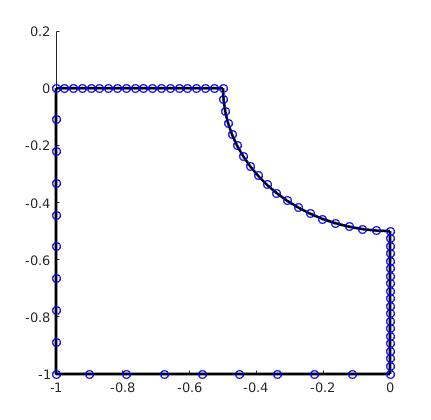
\includegraphics[scale=0.5]{./imgs/img_geometry.jpg}
			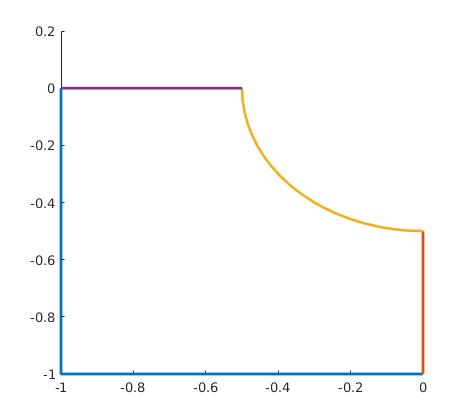
\includegraphics[scale=0.5]{./imgs/img_geometry_boundaries.jpg}
			\caption{Geometr\'ia de prueba}
			\label{fig:img_geometry_boundary}
		\end{figure}
		Esta geometr\'ia est\'a dada en forma de puntos, por lo que no tenemos expresiones anal\'iticas para las fronteras.
		Para esto, expresamos las fronteras como funciones lineales en trozos, haciendo que cada frontera sea definida por un conjunto de subfunciones tipo segmento de recta definidas por los puntos que definen la frontera. Esto se expresa como lo siguinte:
		\begin{gather*}
			x(q) = 
			\begin{cases}
				x_{i}(q) = x(i) + q \lbrace x(i + 1) - x(i) \rbrace
			\end{cases}
			\\
			y(q) = 
			\begin{cases}
				y_{i}(q) = y(i) + q \lbrace y(i + 1) - y(i) \rbrace
			\end{cases}
			\\
			q = {\xi, \eta}
		\end{gather*}
		%
		Al aplicar este m\'etodo a la geometr\'ia dada, obtenemos los siguientes resultados.
		\begin{figure}[H]
			\centering
			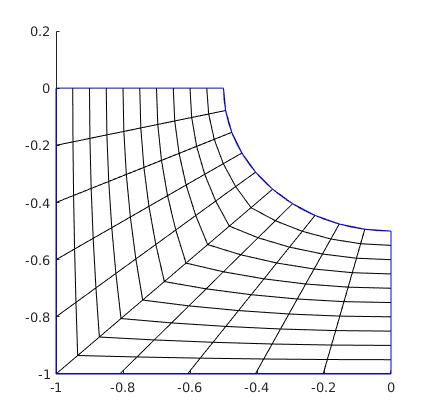
\includegraphics[scale=0.5]{./imgs/img_alg_generator_size_10.jpg}
			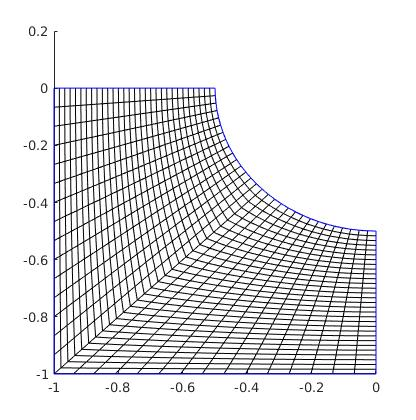
\includegraphics[scale=0.5]{./imgs/img_alg_generator_size_30.jpg}
			\caption{Grid generado para la geometr\'ia de prueba usando el m\'etodo algebraico, size de 10 y 30}
			\label{fig:img_grid_algebraic}
		\end{figure}
		%
		\item[b)] \textbf{ M\'etodo basado en PDEs el\'ipticas }
		\\
		Para poder refinar la malla generada por el generador algebraico usamos un generador basado en PDEs. El generador es del tipo el\'iptico, el cu\'al define la nueva grilla como la soluci\'on a la siguiente PDE :
		\begin{gather*}
		%
			\xi_{xx} + \xi_{yy} = 0 \\
			\eta_{xx} + \eta_{yy} = 0 \\
		%
		\end{gather*}
		\'Estas PDEs las transformamos del espacio $x,y$ al espacio $\xi, \eta$, lo cu\'al nos deja un problema de frontera ( con fronteras $x(\xi,\eta)$, $y(\xi,\eta)$ ) definido por las siguientes ecuaciones :
		\begin{gather*}
		%
			( x_{\eta \eta}^{2} + y_{\eta \eta}^{2} )x_{\xi \xi} 
				- 2 ( x_{\xi} x_{\eta} + y_{\xi} y_{\eta} ) x_{\xi \eta}
				+ ( x_{\xi \xi}^{2} + y_{\xi \xi}^{2} )x_{\eta \eta} 
			\\
			( x_{\eta \eta}^{2} + y_{\eta \eta}^{2} )y_{\xi \xi} 
				- 2 ( x_{\xi} x_{\eta} + y_{\xi} y_{\eta} ) y_{\xi \eta}
				+ ( x_{\xi \xi}^{2} + y_{\xi \xi}^{2} )y_{\eta \eta} 
		%
		\end{gather*}
		%
		Al discretizarlas obtenemos las siguientes ecuaciones :
		\begin{gather*}
			\alpha_{ij} ( x_{i+1,j} - 2 x_{i,j} + x_{i-1,j} ) + \gamma_{ij} ( x_{i, j + 1} - 2 x_{i, j} + x_{i,j-1} ) - \hdots \\
				 0.5 \beta_{ij} ( x_{i+1,j+1} - x_{i+1,j-1} - x_{i-1,j+1} + x_{i-1,j-1} ) = 0
			\\
			\alpha_{ij} ( y_{i+1,j} - 2 y_{i,j} + y_{i-1,j} ) + \gamma_{ij} ( y_{i, j + 1} - 2 y_{i, j} + y_{i,j-1} ) - \hdots \\
				 0.5 \beta_{ij} ( y_{i+1,j+1} - y_{i+1,j-1} - y_{i-1,j+1} + y_{i-1,j-1} ) = 0
		\end{gather*}
		\\
		Donde:
		\begin{gather*}
		%
			 \xi = \frac{i}{N_{\xi}},\eta = \frac{j}{N_{\eta}}
			 \\
			 \alpha_{ij} = 0.25 ( ( x_{i,j+1} - x_{i,j-1} )^{2} + (y_{i,j+1} - y_{i,j-1})^{2} )
			 \\
			 \beta_{ij} = 0.25 ( ( x_{i,j+1} - x_{i,j-1} ) ( x_{i+1,j} - x_{i-1,j} ) + ( y_{i,j+1} - y_{i,j-1} ) ( y_{i+1,j} - y_{i-1,j} ) )
			 \\
			 \gamma_{ij} = 0.25 ( ( x_{i+1,j} - x_{i-1,j} )^{2} + (y_{i+1,j} - y_{i-1,j})^{2} )
		%
		\end{gather*}
		%
		Para resolver estas ecuaciones y transformarlas a un sistema lineal hacemos uso de la iteraci\'on de Picard, haciendo que los coeficientes $\alpha, \beta, \gamma$
		sean dependientes de la malla actual, mientras que los otros t\'erminos sean dependientes de la malla siguiente, teniendo lo siguiente ( caso $x$ ) :
		\begin{gather*}
			\alpha_{ij}^{k} ( x_{i+1,j}^{k+1} - 2 x_{i,j}^{k+1} + x_{i-1,j}^{k+1} ) + \gamma_{ij}^{k} ( x_{i, j + 1}^{k+1} - 2 x_{i, j}^{k+1} + x_{i,j-1}^{k+1} ) - \hdots \\
				 0.5 \beta_{ij}^{k} ( x_{i+1,j+1}^{k+1} - x_{i+1,j-1}^{k+1} - x_{i-1,j+1}^{k+1} + x_{i-1,j-1}^{k+1} ) = 0
		\end{gather*}
		Con lo cu\'al podemos formar el sistema $Az = b$, donde $A$ es la forma matricial de las ecuaciones anteriores luego de aplicar el stencil mostrado en la figura siguiente, $z$ es la representaci\'on en vector columna de la grilla en la siguiente iteraci\'on-refinamiento y $b$ se obtiene de aplicar las condiciones de frontera.
		\begin{figure}[H]
			\centering
			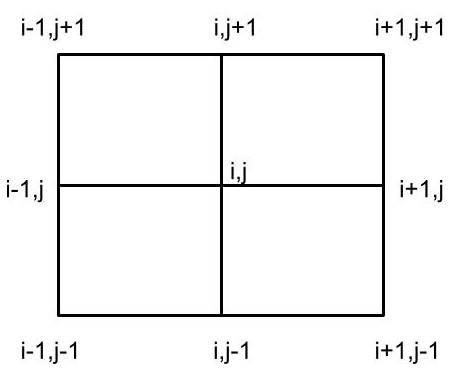
\includegraphics[scale=0.5]{./imgs/img_stencil.jpg}
			\caption{Stencil a aplicar a las ecuaciones discretizadas del generador el\'iptico}
			\label{fig:img_stencil}
		\end{figure}
		Implementamos el generador el\'iptico en MATLAB, lo cu\'al nos dio los siguientes resultados al usar la malla del generador algebraico de la geometr\'ia de ejemplo como condici\'on inicial.
		\begin{figure}[H]
			\centering
			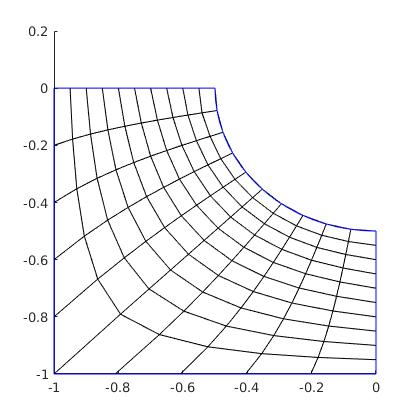
\includegraphics[scale=0.5]{./imgs/img_elliptic_generator_size_10.jpg}
			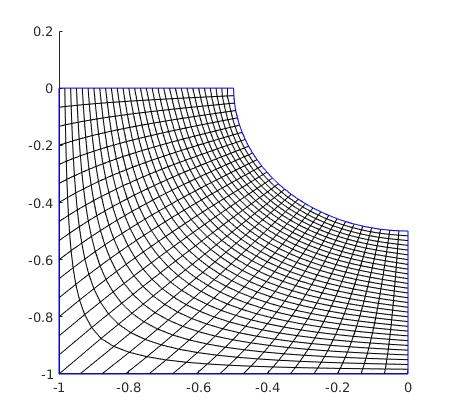
\includegraphics[scale=0.5]{./imgs/img_elliptic_generator_size_30.jpg}
			\caption{Grid generado para la geometr\'ia de prueba usando el generador el\'iptico, size de 10 y 30}
			\label{fig:img_grid_algebraic}
		\end{figure}
	\end{itemize}

% Comentatios finales sobre la estructura de las matrices del sistema.

%%%%%%%%%%%%%%%%%%%%%%%%%%%%%%%%%%%%%%%%%%%%%%%%%%%%%%%%%%%%%%%%%%%%

%%%%%%%%%%%%%%%%%%%%%%%%%%%%%%%%%%%%%%%%%%%%%%%%%%%%%%%%%%%%%%%%%%%%%%%%%%%%%%%%%%%%%%%%%%%%%%%%%%%%%%%%%%%%%%%%%%%%%%
\end{itemize}

%%%%%%%%%%%%%%%%%%%%%%%%%%%%%%%%%%%%%%%%%%%%%%%%%%%%%%%%%%%%%%%%%%%%%%%%%%%%%%%%%%%%%%%%
\end{enumerate}
\end{document}